% Section content template for individual Educative lessons
% This file contains the actual content for a specific section
% Generated from Educative API section content

% Section: Requirements for Stack Overflow
% Section ID: 4681614011662336
% Section Slug: requirements-for-stack-overflow
% Generated: 2025-12-12T22:49:03.823178

In this lesson, we'll list Stack Overflow's requirements. This is a crucial step, as requirements define the scope of a problem. Getting them right from the interviewer and understanding them well will make the design of the rest of the system smooth and easy.
\\
We'll use the notational convention to identify each requirement with a unique label ``Rn,'' where ``R'' is short for requirement and ``n'' is a natural number.

\subsection{Requirement collection}\label{_Icwm3boS1yx3LfVja6o1}
\\
The requirements for Stack Overflow are defined below:

% \vspace{-1.0\baselineskip}
\noindent
\begin{minipage}[t]{0.48\textwidth}\vspace{0pt}
\textbf{R1:} Any guest can view and search questions by tag, username, or word.
\\
\textbf{R2:} Users should be able to add new questions and add answers to an open question.
\end{minipage}
\hfill
\begin{minipage}[t]{0.48\textwidth}\vspace{0pt}
\centering
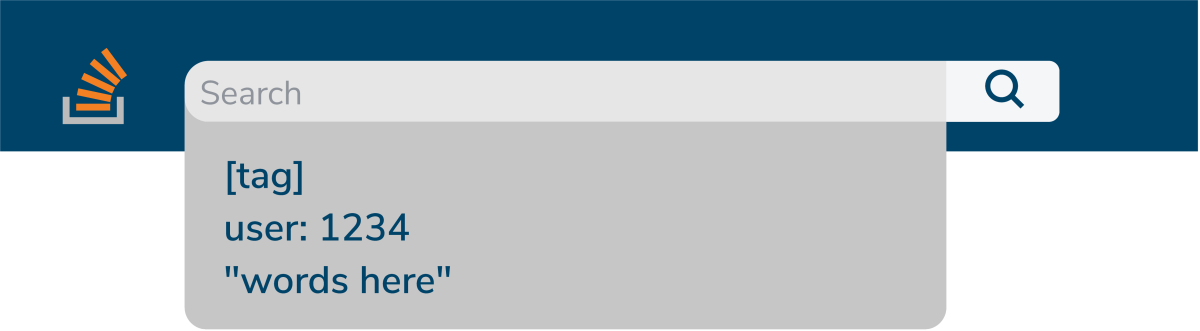
\includegraphics[width=0.5\textwidth]{Images/chapter_20/section_4681614011662336/5878635519279104.png}
\end{minipage}

% \vspace{-1.0\baselineskip}
\noindent
\begin{minipage}[t]{0.48\textwidth}\vspace{0pt}
\textbf{R3:} Users can flag a question, answer, or comment if anything goes against the community guidelines.
\\
\textbf{R4:} A user can upvote, downvote, and add comments to a question or answer, while they can only upvote a comment.
\\
\textbf{R5:} Users can vote to delete or close off questions for community-specific reasons. However, they can only vote to delete an answer.
\\
\textbf{R6:} Users can add a bounty to their question to attract more answers. A Bounty refers to an award of granting reputation points on a question to attract more attention from other users.
\end{minipage}
\hfill
\begin{minipage}[t]{0.48\textwidth}\vspace{0pt}
\centering

\includegraphics[width=0.5\textwidth]{Images/chapter_20/section_4681614011662336/5579556042047488.png}
\end{minipage}

% \vspace{-1.0\baselineskip}
\noindent
\begin{minipage}[t]{0.48\textwidth}\vspace{0pt}
\textbf{R7:} Moderators can close or restore a deleted question. Moderators can also delete answers.
\\
\textbf{R8:} The system should notify the user whenever there has been an interaction with them, such as the user's question receiving an answer, earning a badge, or someone upvoting or downvoting their post.
\\
\textbf{R9:} Users can earn badges for their helpful answers or comments.
\\
\textbf{R10:} Users can add tags to their questions. A \textbf{tag} is a word or phrase describing the question's topic.
\\
\textbf{R11:} The system should also be able to determine the most popular tags used in questions.
\end{minipage}
\hfill
\begin{minipage}[t]{0.48\textwidth}\vspace{0pt}
\centering

\includegraphics[width=0.5\textwidth]{Images/chapter_20/section_4681614011662336/4864185117966336.png}
\end{minipage}

We've identified our requirements for the problem, and in the next lesson, we will define different use cases of Stack Overflow.

% End of section content